\documentclass[discrete.tex]{subfiles}
 
\begin{document}

\section{АВЛ-деревья}

\begin{definition}
    АВЛ-дерево - сбалансированное по высоте двоичное дерево поиска, для каждой его вершины
    высота ее двух поддеревьев различается не более чем на 1
\end{definition}

\begin{theorem}
    АВЛ-дерево с $n$ ключами имеет высоту 
    \[h = O(\log N)\]
\end{theorem}

\begin{definition}
    Баланс вершины - разница между высотами ее поддеревьев 
\end{definition}

\begin{definition} [Балансировка]
    Балансировка - операция, которая в случае разницы высот левого и правого поддеревьев 
    $\abs{h(L) - h(R)} = 2$, изменяет связи предок-потомок 
    в поддереве данной вершины так, что разница 
    становится $<= 1$, иначе ничего не меняет.\\
    Восстановить баланс можно с помощью поворотов (всего их 4: левый простой, 
    правый простой, левый большой, правый большой)\\
    Простой поворот выполняется при условии $h(s) \leq h(D)$
    \begin{figure}[H]
        \caption{Простой поворот вправо}
        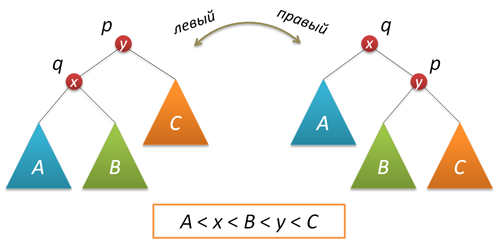
\includegraphics[scale=0.5]{pics/33_1.png}
        \centering
    \end{figure}
    
    \begin{figure}[H]
        \caption{Применение простого поворота}
        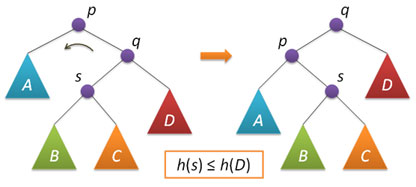
\includegraphics[scale=0.5]{pics/33_2.jpg}
        \centering
    \end{figure}
    Большой поворот выполняется при условии $h(s) > h(D)$ и сводится к двум простым 
    поворотам
    \begin{figure}[H]
        \caption{Большой поворот}
        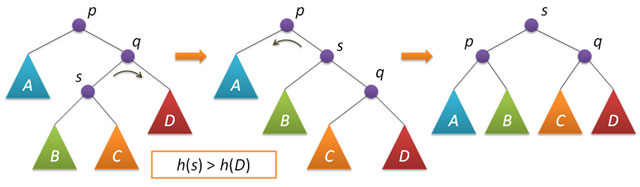
\includegraphics[scale=0.5]{pics/33_3.jpg}
        \centering
    \end{figure}
    hint: первым простым поворотом мы отменяем это условие

\end{definition}

\begin{definition} [Добавление вершины]
    Добавляем вершину как в бинарном дереве. Спускаемся вниз, как при поиске ключа t.
    Если мы стоим в вершине $a$ и нам надо идти в поддерево, которого нет, то делаем 
    ключ t листом, а вершину $a$ его корнем. \\
    Дальше поднимаемся вверх и пересчитываем баланс у вершин. 
    Если мы поднялись в вершину $i$ из левого поддерева, то 
    баланс $i$ - ой вершины увеличивается на 1, иначе уменьшается.\\
    Если мы пришли в 
    вершину и ее баланс $ = 0$ после пересчета, то это значит, что высота поддерева с 
    корнем в этой вершине не изменилась, можно остановить подъем.\\
    Если баланс вершины после пересчета $= -2 $ или $ 2$, то нам необходимо сбалансировать
    это поддерево.\\
    \\
    Добавление работает за $O(\log n)$, т.к. мы рассмотрим не больше, чем $O(h)$ 
    вершин

\end{definition}

\begin{definition} [Удаление ключа]
    \begin{enumerate}
        \item найдем удаляемый ключ p в дереве (если не нашли, то ничего не делаем)
        \item в правом его поддереве найдем наименьший элемент min
        \item поменяем местами поменяем местами p и min
        \item удалим p
        \item сбалансируем все, что выше p
    \end{enumerate}
    \begin{figure}[H]
            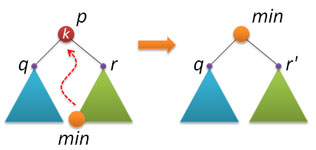
\includegraphics[scale=0.5]{pics/33_4.jpg}
            \centering
    \end{figure}
    При удалении возможна ситуация, когда вершина p не имеет правого поддерева, тогда
    по св-ву АЛВ-дерева либо эта вершина имеет слева единственный дочерний узел,
    либо она является листом. В обоих случаях мы просто удаляем p и возвращаем указатель
    на левое поддерево.
\end{definition}

\end{document}
